\section{Voronoi}
The current best model uses k-means clustering of of the points to the center points. For every point (the plane is seen as a finite number of pixels) in the plane, $p$, it finds the seed point, $s_i$, which is the shortest distance to it, i.e. such that $\sqrt{\big(p(x)-s_i(x)\big)^2 + \big(p(y)-s_i(y)\big)^2}$ is minimum. This is suboptimal as the time taken to create the diagram relies on the dimensions of the plane and the number of seed points in it. Instead we seek a method which is invariant of the plane size and relies solely on the seed points, for the sake of increasing the computation time, this method must also be parallelizable. 
\\
\\
It was therefore decided that the divide and conquer method (Chapter \ref{tes:ssec:dac}) would be used. The algorithm works by ordering the points, first by their $x$ then their $y$ values. The points are then divided into two subsets, a left and right set. The Voronoi diagrams are then generated for the left and right subsets using the divide and conquer method. The convex hulls of the left and right Voronoi diagrams are then found. The lowest common support line between the hulls is then found and from this a dividing polygonal chain is generated until it intercepts the upper bounds of the plane. The intersecting edges with the polygonal chain are then determined, and cut so that part of the chain is now part of the Voronoi cells edges.
\\
\\
Code for the Divide and Conquer was adapted from that in the git repository pyVoronoi\footnote{https://github.com/twmht/pyVoronoi}. pyVoronoi is an implementation for the Divide and Conquer Voronoi algorithm written in python 2.7. pyVoronoi uses a simple GUI to generate a voronoi diagram in a fixed plane using sources read in from a text file. This interface, while simple to use, is constraining as it does not allow the user to specify their own spacial constrains or generate the voronoi as part of a pipelined process. The visualiser and interface were therefore removed and the remaining code re-factored so that the process is a function which may be called by the user or used in a larger process.

\subsection{Structures of the Voronoi}
The voronoi structure is mainly made up of two structures, lines and points. Points are mainly used to define the sources, but are also used to generate line. Points are made up of an x, y and z value, which determines the position and intensity of the point. Each point also has a circumcentre attribute to determine whether it is the point of intercept of three lines (this is most commonly used in the points at the end of a line), two point parameters to indicate the points on either side of the point if the point lies on the convex hull, these are initialised as None, a list of related structures containing another point and their corresponding bisecting line, this list is set as empty. The point also has a list of all the sources contained in the cell and an error value associated to it, these values are set to an empty list and zero respectively and will only come into use after the voronoi diagram has been generated.
\\
\\
A line is made up of two points which define its endpoints, if the line is a bisector it contains two more points which define the source points used to generate it, if not these values are set to None. The line also contains a list of all the other lines the line is connected to as well. The line finally has an availability boolean parameter which defines whether or not the line is actively available to intercept with other lines or if it has been discarded from the overall voronoi structure.

\subsection{Voronoi Function}

The Voronoi function takes in the list of points and a range of points it will operate on (initially the entire set of points). Depending on the number of points in the subset range, one of four operations will occur. If the range is made up of more than three points, the range is divided into two equal sub ranges, one from the starting point of the range to the median and another from the point after the median to the end of the range. The Voronoi function is then called again for each sub range, denoted as VDL and VDR for left and right sub ranges respectively, with the full set of points. Once the voronoi structure for these two are calculated, the merge function is called with VDL and VDR and the function ends as it is not value returning.
\\
\\
If the range is three, the function generates three lines, one for the each pair of the three point. The intercepts of the lines is determined, if it does not exist, an invalid line exists, this line is found and removed. If the intercept does exist, it is found and the lines are clipped at the intercept. The lines are listed and returned with the range and the corresponding convex hull structure made up of all three points.
\\
For a range of two points, the bisecting line is determined as the only line in the structure. The line is placed in a list where it is the only element and along with the point range and the convex hull, only made up of the two points, are returned.
\\
The case of a single point is excluded as the first case of multiple points being divided in two equal or near equal sets and the case of three and two points in a set will make the case of a single point impossible.

\subsection{Convex Hull}
Andrew's monotone chain convex hull algorithm was used to determine the convex hull of a set of points. The function is first passed a range of points on which to operate. The points must be ordered lexicographically (first by the x coordinate then by y if there is a tie), which they are as this is needed for generating the voronoi structure. A list of zeros, twice the size of the number of points in the range is generated, this list will hold the elements of the chain. The complete convex hull is calculated in two steps, the first finds the upper hull and the second, the lower hull.
\\
The first point (the leftmost) and the second point in the range are added to the list. We then iterate over the rest of the range, adding the next point to our list, if the angle created by these three points is less than $\pi$ radians, the points are left in the list, the next point in the range is added and the three latest points in the list are analysed for their angle again until we reach the. If the angle is greater than $\pi$ radians, the two latest points in the list are removed and the process continues. This generates the upper hull of the convex hull.
\\
To generate the lower hull, the same process is used, but the range is iterated over in reverse, starting at the rightmost point and ending at the leftmost.
\\
One the list is populated with the points of the lower and upper hulls, they form the monotone chain. The chain is then iterated over and each point in the chain adds the preceding point to its fifth parameter and the next point to its fourth.

\subsection{Voronoi Merge Function}
The merge begins by finding the upper and lower tangents of the VDL and VDR sets. These tangent lines are defined as connections between the convex hulls of VDL and VDR with a point in each as the endpoints of the line. Starting from the rightmost point in VDL and the leftmost in VDR, it finds the upper tangent by finding the pair of points (one in VDL and one in VDR) who, together with their respective adjacent points, both generate an angle less than $\pi$ radians, the order and the adjacent point being used is counter-clockwise for VDL and clockwise for VDR. To find the lower tangent, the order is reversed with VDL stepping clockwise and VDR counter-clockwise.
\\
The upper tangent is used to find the starting point of the polygonal chain used to merge the voronoi. Bisector of the endpoints of the line, which both lie on convex hulls, are used as the first line segment in the chain which is appended to a list of lines called HP. The uppermost of the two points in the upper tangent is determined and a new tangent is generated with the lower point and the uppermost point's neighbour, not necessarily in the convex hull, so long as it is not a convex hull neighbour of the lower point and it's related line to the upper point is both available and intercepts the bisector of the upper tangent. The bisecting line of the new point which intercepts the new bisector along with the new bisector itself is added to a list of lines to be clipped, clip\_lines. The same set of operations then occur with the new point and the lower of the upper tangent defining the new tangent. This continues until the bisecting line of the lower tangent is determined. Once complete, we are left with a list, HP, which contains the bisecting lines between points in VDL and VDR and a list of bisecting lines from VDL and VDR together with lines from HP, clip\_lines. The lines in clip\_lines and HP are both cut at their intercepts and all are appended to a list of lines to be passed back along with the range of points and the new convex hull of the combined voronoi structure.
\\
\\
An Example of the Voronoi Tessellation can be seen in Figure \ref{fig:gen_voronoi}
\begin{figure}[H]
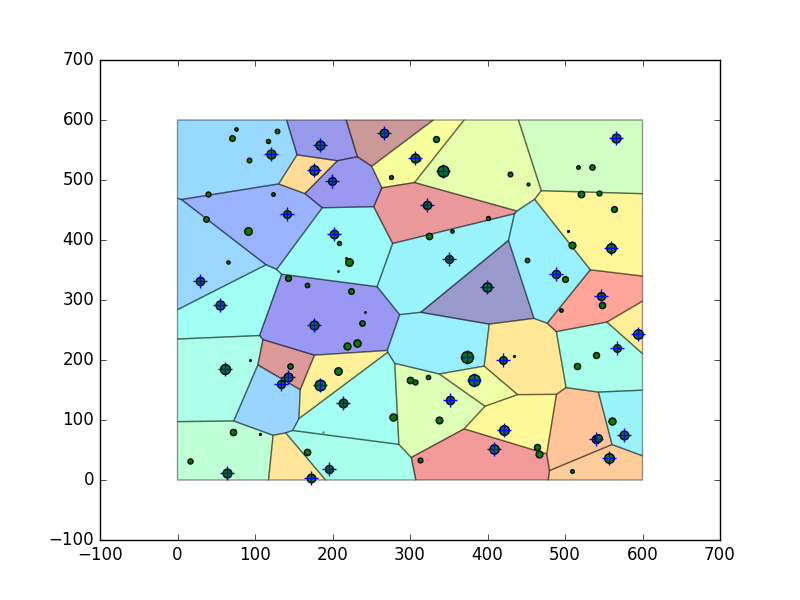
\includegraphics[width=\textwidth]{Images/recentre1.png}
\caption{A Generated Voronoi Tessellation.}
\label{fig:gen_voronoi}
\end{figure}
\subsection{Weighted Voronoi Tessellation}
An attempt was made to generate a weighted Voronoi tessellation using a distance transform which uses the intensities of the centres to redetermine the coordinates of the midpoint of the centres, this transform can be seen in equation \ref{eq:w_dist} where $z_1$ and $z_2$ are the intensities of $\vec{x_1}$ and $\vec{x_2}$ respectively.
\begin{equation}\label{eq:w_dist}
	d'(\vec{x_1},\vec{x_2}) = \frac{z_1}{z_1+z_2}\vec{x_1} + \frac{z_2}{z_1+z_2}\vec{x_2}
\end{equation}
This is an extension of the standard distance equation since, if $z_1=z_2$ we obtain
\begin{align*}
	d'(\vec{x_1},\vec{x_2}) &= \frac{z_1}{z_1+z_2}\vec{x_1} + \frac{z_2}{z_1+z_2}\vec{x_2} \\
	d'(\vec{x_1},\vec{x_2}) &= \frac{1}{2}\vec{x_1} + \frac{1}{2}\vec{x_2} \\ 
	d'(\vec{x_1},\vec{x_2}) &= \frac{\vec{x_1} + \vec{x_2}}{2} \\
\end{align*}
Some complications were found in this, namely on the convex hull. Weighted centres which are not on the hull but due to their larger weighting still have cells which dominate areas of the hull. This leads to them not being included in the merging process and their line segments not being clipped or deactivated. Another problem with this is that it generates undefined regions in the space, regions where domains overlap due conflicting weightings, an example of this can be seen in Figure \ref{fig:w_voronoi_issue}.
\begin{figure}[H]
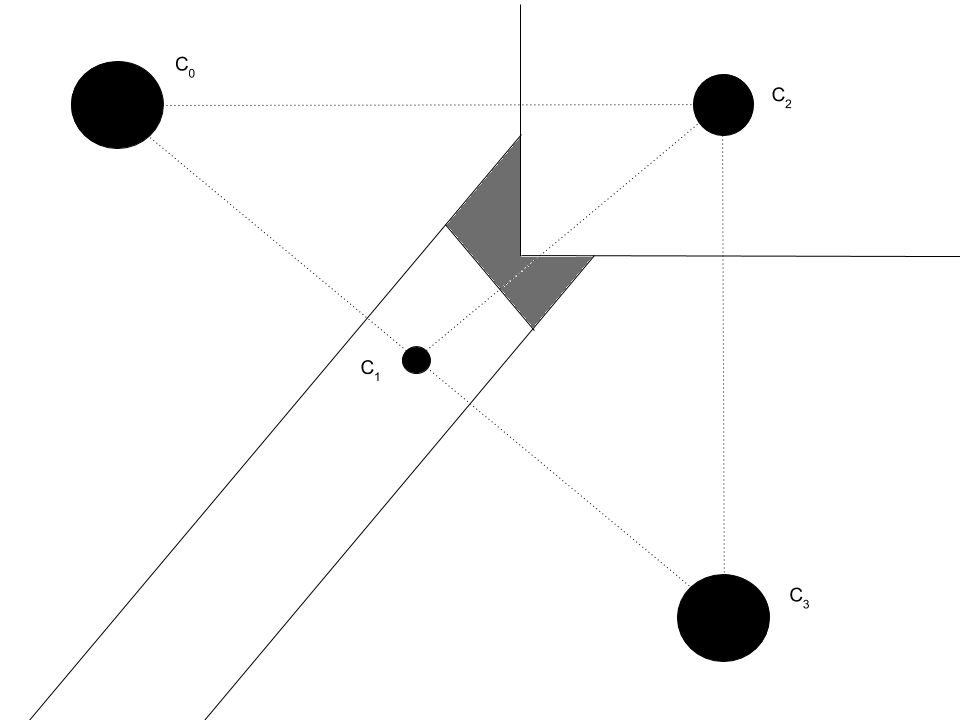
\includegraphics[width=0.5\textwidth]{Images/weighting_problem.png}
\centering
\caption{An unclassified area (grey) generated by a weighting conflict in $c_1$ and $c_2$.}
\label{fig:w_voronoi_issue}
\end{figure}
It shows a conflicting area between $c_1$ and $c_2$, it should be expected that $c_2$, with its higher intensity, should claim the area, but in doing so it will cross into what then should be the domain of $c_0$ or $c_3$. It was for this reason that the choice to use the intensities to weight the Voronoi tessellation generated was abandoned and that the intensities would rather be used for calculating the error and calculating cell merges. An example of a failed weighted Voronoi tessellation can be seen in Figure \ref{fig:w_voronoi}.
\begin{figure}[H]
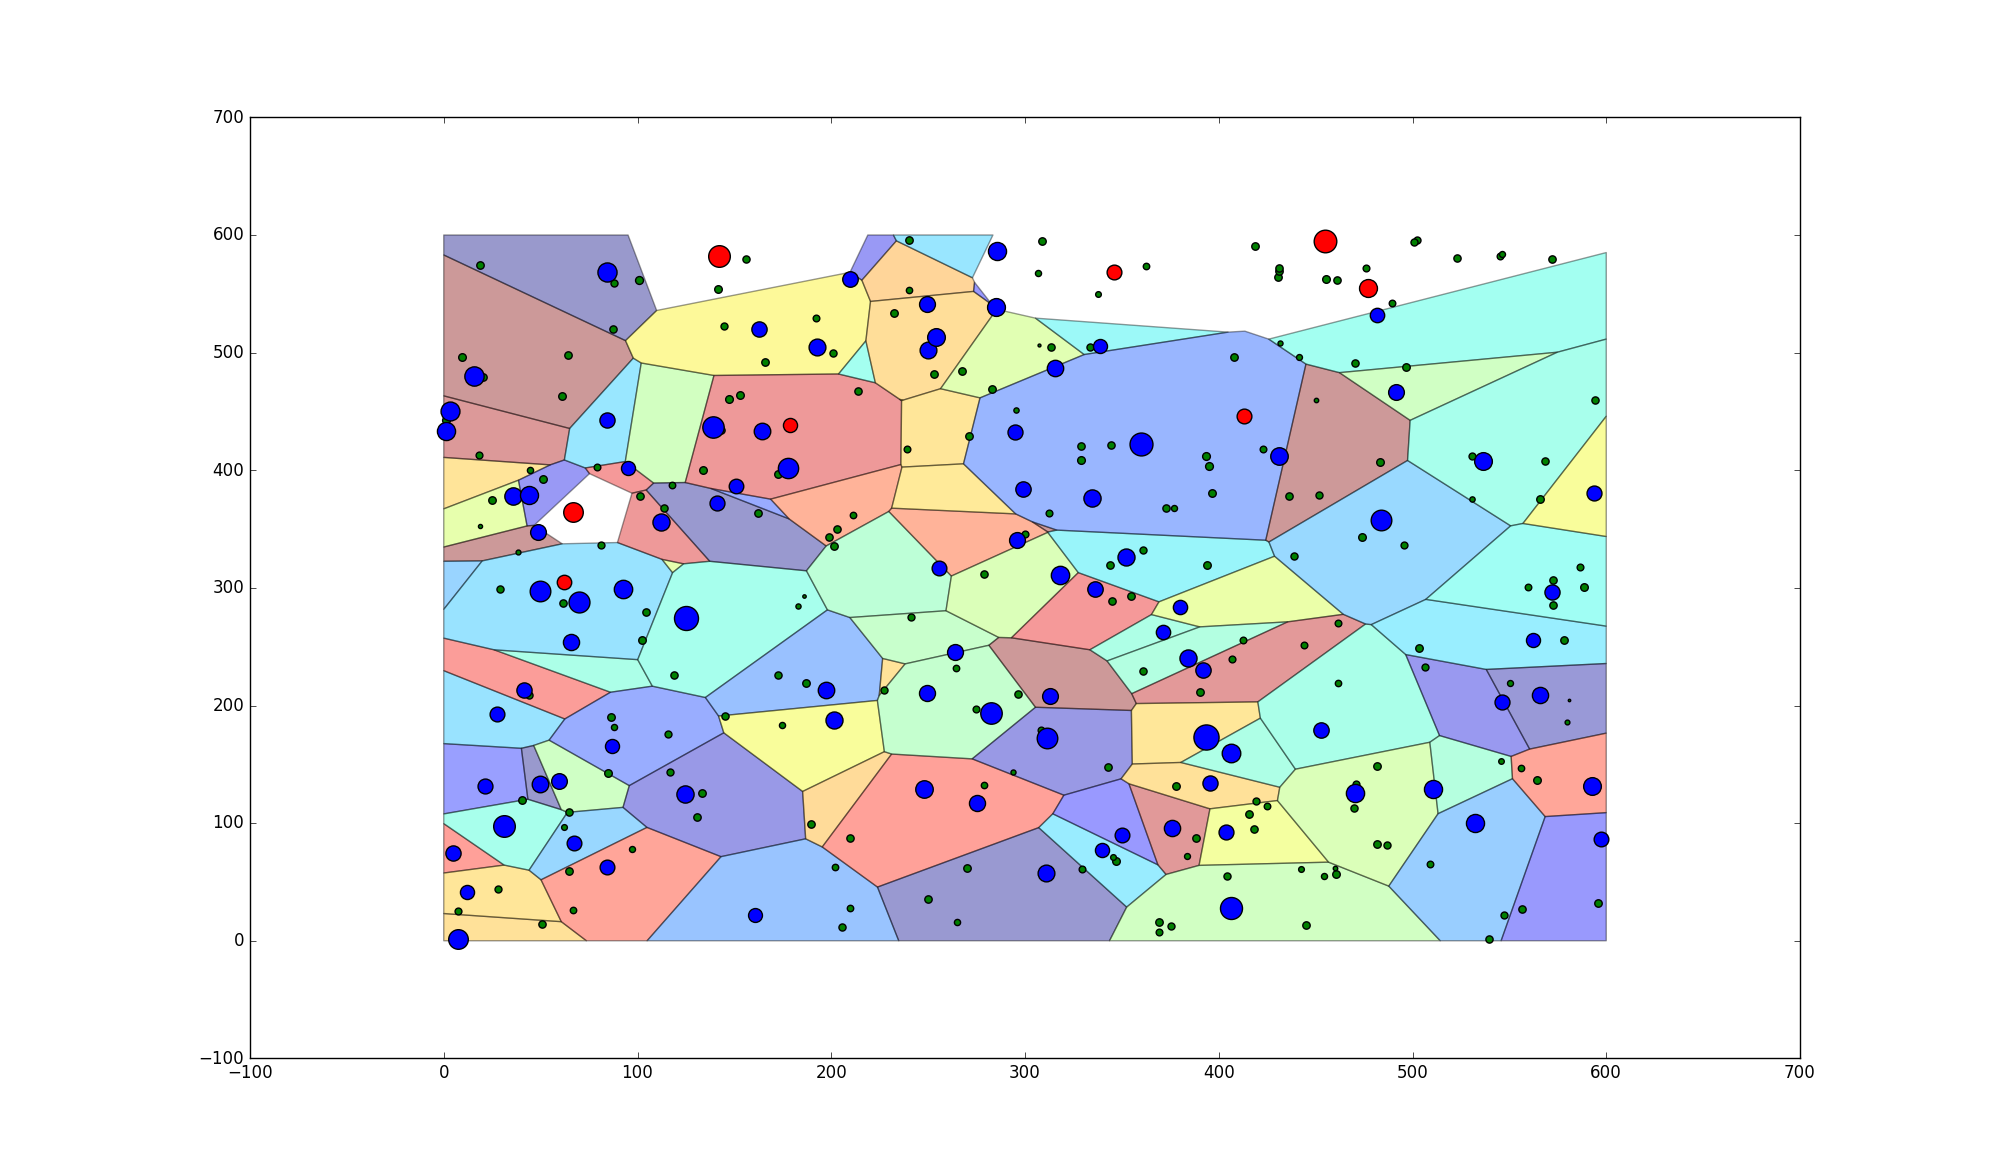
\includegraphics[width=\textwidth]{Images/weighted_voronoi.png}
\centering
\caption{A failed visualisation of a weighted Voronoi tessellation.}
\label{fig:w_voronoi}
\end{figure}